Darwin's theory of evolution through natural selection has been a cornerstone of
biology for over a century and half. Yet, a quantitative theory of complexity
that could arise through Darwinian mechanisms has remained virtually unexplored.
To address this question, Valiant introduced a computational model of
evolution~\cite{Valiant:2009-evolvability}.
In his model, an organism is an entity that computes a function of
its environment.  There is a (possibly hypothetical) \emph{ideal function}
indicating the best behaviour in every possible environment. The performance of
the organism is measured by how close the function it computes is to the ideal.
Mutations may alter the function computed by an organism and the performance
(fitness) measure forms the basis of natural selection. The resources allowed
are the most generous while remaining feasible; the mutation mechanism may be
any efficient randomised Turing machine, and the function represented by the
organism may be arbitrary as long as it is computable by an efficient Turing
machine.

Formulated this way, the question of evolvability can be asked in the language
of computational learning theory. For what classes of ideal functions, $C$, can
one expect to find an evolutionary mechanism that gets arbitrarily close to the
ideal, within feasible computational resources? Darwinian selection is
restrictive in the sense that the only feedback received is aggregate over life
experiences. Valiant observed that any feasible evolutionary mechanism could be
simulated in the statistical query framework of Kearns~\cite{Kearns:1998}. In a
remarkable result, Feldman~\cite{Feldman:2008-evolvability} showed that in fact,
evolvable concept classes are exactly captured by a restriction of Kearns's
model, where the learning algorithm is only allowed to make \emph{performance
queries}, \ie it produces a hypothesis and then makes a query to an oracle that
returns the (approximate) performance of that hypothesis under the
distribution.\footnote{Feldman calls these queries correlational statistical
queries, because when working with Boolean functions with range $\{-1, 1\}$, the
performance of any hypothesis is its correlation with the ideal function.} P.
Valiant studied the evolvability of real-valued functions, and showed that
whenever the corresponding weak optimisation problem, \ie approximately
minimising the expected loss, can be solved by using a weak-evaluation oracle,
such an algorithm can be converted into an evolutionary
mechanism~\cite{Valiant:2012-real}. This implies that a large of class of
functions -- low degree real polynomials -- can be evolved with respect to any
convex loss function.
%%
\eat{
Direct evolutionary mechanisms \dots \eanote{Summarize what these are and what
they achieve -- I don't totally understand what ``direct'' means.} }
%%

Direct evolutionary mechanisms, not invoking the general
reduction of Feldman and P. Valiant, have been proposed for certain classes in
restricted settings. Valiant~\cite{Valiant:2009-evolvability} showed that the
class of disjunctions is evolvable using a simple set of mutations under the
uniform distribution. Kanade, Valiant and Vaughan proposed a simple mechanism
for evolving homogeneous linear separators under radially symmetric
distributions~\cite{KVV:2010-drift}.  Feldman considered a model where the ideal
function is boolean but the representation can be real-valued, allowing for more
detailed feedback. He presents an algorithm for evolving large margin linear
separators for a large class of convex loss functions~\cite{Feldman:2011-LTF}.
P. Valiant also showed that with very simple mutations, the class of low-degree
polynomials can be evolved with respect to the squared
loss~\cite{Valiant:2012-real}.

The more direct algorithms are somewhat appealing due to the simplicity of their
mutations.  However, a meaningful definition of \emph{naturalness} of mutations
would be hard to make.
Another desirable property of some of these more direct algorithms is that the
representations used are functions of low complexity. Feldman's general
reduction from statistical query algorithms may use arbitrarily complex
representations (polynomial-sized circuits) depending on the specific algorithm
used. The ``chemical computers'' of organisms may be slow, and hence,
representations that have low-complexity are attractive. We first describe a
particular class of biological circuits, \emph{transcription networks}, that
motivate our study. We then frame the question in the language of computational
learning theory, summarize our contributions and discuss related work.

\eat{ \todovk{I'd like this paragraph re-worded.} \todoea{I think much of this
paragraph could be deleted.}

Modeling mutations as the outputs of a Turing machine offers appealing
generality that captures a fundamental notion of the evolvable that is not
specific to life on Earth, \eg, requiring that creatures use sequences of DNA to
represent their hypotheses.  At the same time, the more direct algorithms are
appealing because \dots \eanote{Because of their ``naturalness''?} However, it
is difficult to define what constraints ``naturalness'' might place on
mutations.  Our current understanding of biological mutations and the
relationship between genotype -- the representation of a hypothesis -- and
phenotype -- its corresponding functional output -- is incredibly limited.
Thus, Valiant~\cite{Valiant:2013-PAC} argued that a temptation to define
\emph{naturalness} should be resisted, \eanote{while observing that natural
systems are constrained?} In this work, we suggest that the other general aspect
in Valiant's model, \eanote{What is the first general aspect?} representations
being arbitrary polynomial-time computable functions, may indeed benefit from a
closer study of biology.  }

\subsection{Representation in Biology}

\eat{
\vknote{ \emph{We should talk about this a bit more. I don't know whether it's
worth talking about bounded functions. But may be you'll point me to the
write-up from Paul's paper. Ok - this part of biology, I'm not comfortable
handling. Let's talk more. Concluding interactions from sparsity may be a bit
trickier. To be fair, that's also the case with transcription networks we'll
talk about below, but probably less so.} Biological systems appear to function
successfully with greatly restricted representation classes. For example, one
natural restriction is that concept classes ought to be bounded. P. Valiant
argues that since selection can only act on polynomially many offspring per
generation, evolution can only reasonably approximate bounded (real) numbers in
polynomial time~\cite{Valiant:2012-real}.  We study additional restrictions
motivated by physical constraints on genes and proteins within a cell.  Consider
\emph{Escherichia coli}, a single-celled bacterium that has thrived for millions
of years in the digestive systems of animal hosts; its responses to the
environment -- which is dynamic and very high-dimensional -- are specified in
about 4,000 genes~\cite{biology}. As in other organisms, these genes encode
proteins that interact with the environment, with each other and with genetic
material to regulate cellular function (Figure~\ref{}). At any particular
moment, each protein can physically interact with only a small number of other
molecules -- other proteins, DNA or other molecules, \eg sugars or toxins.
Consequently, a ubiquitous property of these interaction networks is sparsity
\eanote{that something something\dots} }
}
Biological systems appear to function successfully with greatly restricted
representation classes. The nature of circuits found in biological systems may
vary, but some aspects -- such as \emph{sparsity} -- are common.
Specifically, the interacting components in many biological circuits are
sparsely connected. Biological circuits are often represented as networks or
graphs, where the vertices correspond to entities such as neurons or molecules
and the edges to connections or interactions between pairs of entities.
For example, both neural networks~\cite{Watts:1998} and
networks of metabolic reactions in the cell~\cite{Wagner:2001,Barabasi:2000}
have been described by ``small-world'' models,
where a few ``hub'' nodes have many edges but most nodes have few edges
(and consequently, the corresponding graphs have small diameter).
An associated property observed in biological networks is \emph{modularity}:
a larger network of interacting entities is composed of smaller modules of
(functionally related) entities~\cite{Hartwell:1999}.
%It has been shown that in networks of interacting proteins, ``hub'' nodes
%tend not to be connected to each other but rather to low-degree
%nodes~\cite{Maslov:2002} and further that there exist smaller modules with many
%internal connections but few connections to the larger
%network~\cite{Mirny:2003}.
%functional localization arises through
%molecular specificity~\cite{Schrodinger:1944,Kauffman:1969},
%spatial localization, or temporal localization
Both the ``small-world'' description and modularity of biological networks are
consistent with the more general theme of sparsity.

\begin{figure}[ht]
\centering
\subfigure[~]{
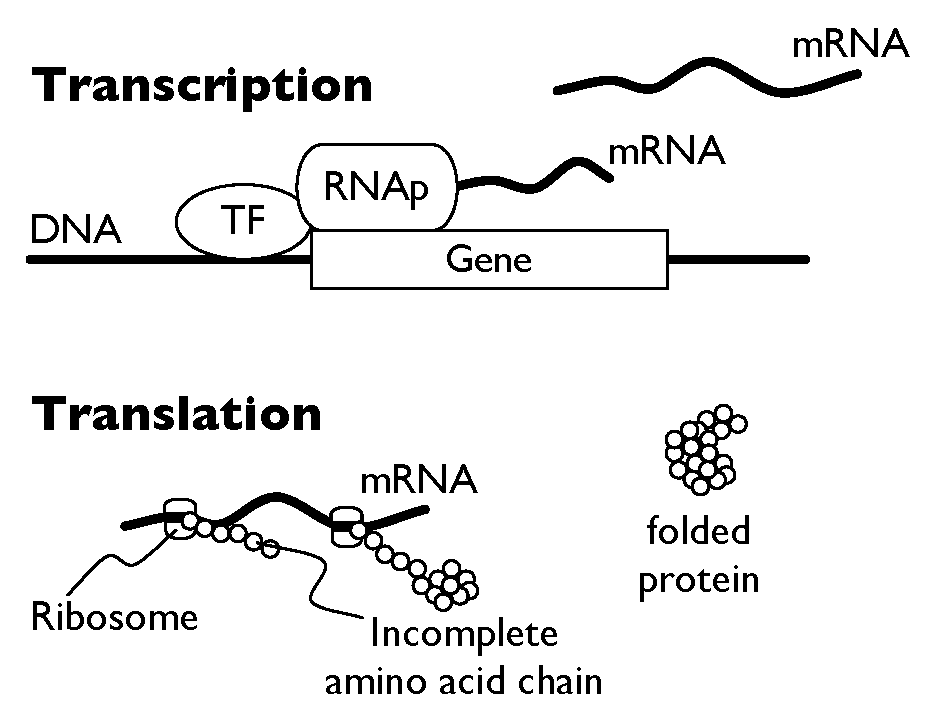
\includegraphics[width=0.5\textwidth]{figs/biology}
\label{fig:biology}
}
%\hspace{0.2in}
\subfigure[~]{
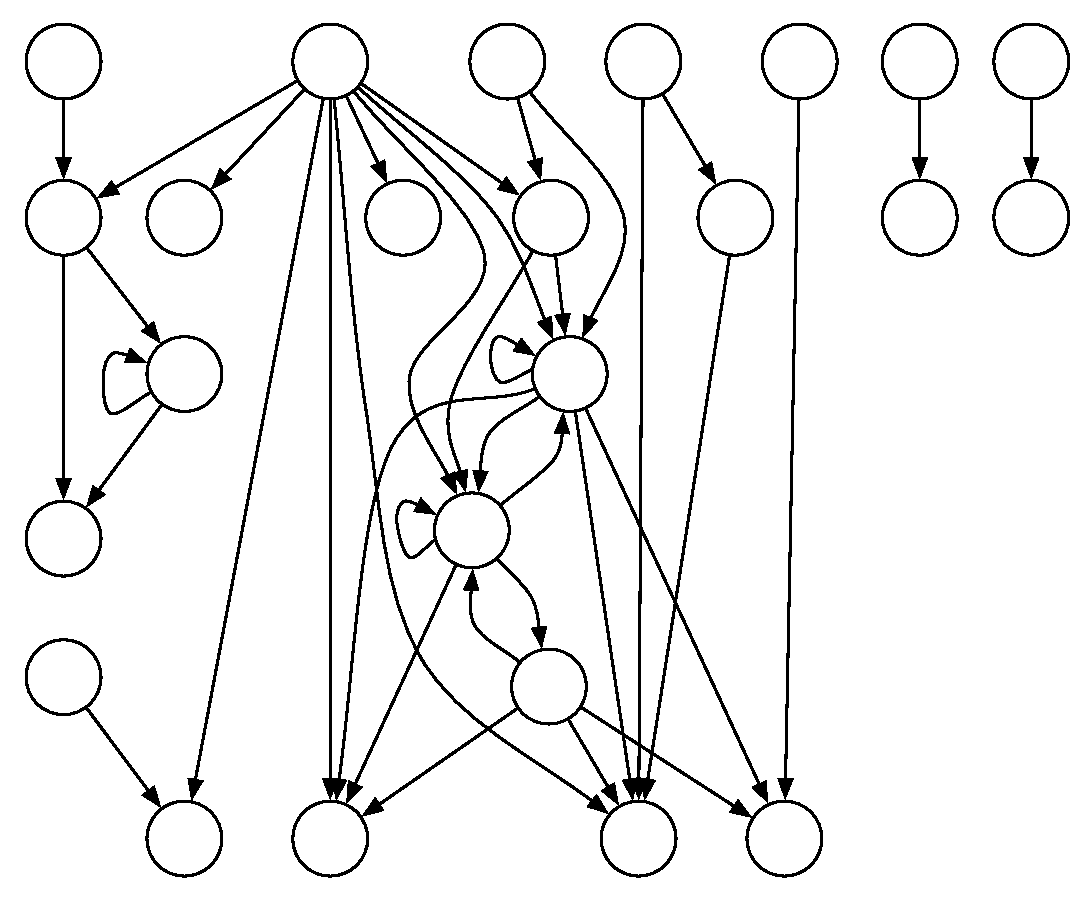
\includegraphics[width=0.45\textwidth]{figs/network}
\label{fig:network}
}
\caption{(a)~Schematic of transcription (top) and translation (bottom).
Here, a transcription factor (TF) binds to DNA close to a gene in a way that
increases gene expression by encouraging RNA polymerase (RNAp) to transcribe
the gene and so produce mRNA.  The mRNA is then translated by ribosomes to
produce sequences of amino acid that ultimately fold into proteins.
Due to physical limitations, only a small number of transcription factors can
directly regulate any gene. Note that a transcription factor's action can also
decrease gene expression. For a more complete picture, \eg see~\cite{Alon:2006}.
(b)~Topology of the transcription network of respiration and redox reactions in
yeast. $X \rightarrow Y$ represents that transcription factor $X$ regulates the
expression of $Y$. Note that this real network has cycles.
Adapted from~\cite{Murray:2011}.}
\end{figure}

We focus on transcription networks, which are a specific class of networks of
interacting genes and proteins that are involved in the production of new
protein. For an accessible and mathematical introduction to transcription
networks and other biological circuits, see~\cite{Alon:2006};
below and in Figure~\ref{fig:biology},
we present a simplified account that motivates this work.
In a transcription network, a gene's expression, which is the quantity of the
corresponding protein produced, may be regulated by a set of proteins called
\emph{transcription factors}.\footnote{In reality, this is a dynamical system
and the rate of production also plays a role.  Genes are \emph{transcribed} to
produce mRNA, which is then \emph{translated} into sequences of amino acids
that ultimately fold into proteins.  This process need not be linear:
a gene (mRNA transcript) can be transcribed (translated) multiple times,
not only in series but also in parallel fashion.  For the purposes of this
discussion, we ignore other \emph{epigenetic} effects, \ie molecular
modifications to DNA that do not change its sequence but alter gene expression,
\eg addition of methyl groups to nucleotides in a way that physically blocks
transcription.~\eanote{Does this need a textbook citation?}} These transcription factors
may increase or decrease a gene's expression by binding to regions of DNA close
to the gene. Thus, physical limitations demand that only a small number of
transcription factors may regulate a single gene.  For example, Balaji
\etal~studied a yeast transcription network of 157 transcription factors regulating 
4,410 genes. They observed this network to have 12,873 interactions (edges) where
each gene was regulated on average by about 2.9 transcription factors, the
distribution of in-degrees was well-described by an exponential fit, and only
about 45 genes had an in-degree of 15 or greater~\cite{Balaji:2006}.
%$0-12$~\vknote{Citations: Alon's book and references therein. See pg. 16 Chap 2.}

The number of transcription factors varies from hundreds in a bacterium to
thousands in a human cell. Some transcription factors are always present in the
cell and can be thought of as representing a \emph{snapshot} of the environment.
For example, the presence of sugar molecules in the environment may cause
specific transcription factors to be \emph{activated}, enabling them to regulate
the production of other proteins.  One of these proteins could be an
\emph{end-product}, such as an enzyme that catalyzes a metabolic reaction
involving the sugar. Alternatively, the transcription factor could regulate
another transcription factor that itself
regulates other genes -- we view this as intermediate computation -- and may
participate in further ``computation'' to produce the desired end-result.

While transcription networks may include cycles (loops), here for simplicity we
focus on systems that are directed acyclic graphs, and the resulting computation
can be viewed as a circuit. These circuits are by necessity shallow due to
another physical constraint: the time required for sufficient quantities of
protein to be produced is of the same magnitude as cell-division
time.\footnote{Other kinds of networks, such as signaling networks, operate by
changing the shapes of proteins. The fact that these transformations are rapid may
allow for much larger depth. Note that fast conformational changes govern how
transcription factors directly process information from the environment in order
to regulate gene expression.  In our example, a sugar molecule binds to a
transcription factor and changes its shape in a way that alters its ability to
bind to DNA.}
For example, Luscombe \etal~measured the shortest path length (in number of
intermediate nodes) between transcription factors and regulated genes
corresponding to terminal nodes (leaves) in a yeast transcription network. In
the static network, the mean such path length was 4.7 and the longest path
involved 12 intermediate transcription factors~\cite{Luscombe:2004}.
We illustrate a small, real transcription network in Figure~\ref{fig:network}.

\subsection{Our Contributions}

First, our contribution is conceptual. We believe that the study of evolvability from
a computational standpoint will benefit by understanding the representation
complexity required to evolve a certain concept class. Motivated by the previous
discussion, in the case of transcription networks, it appears essential that the
representation used be a constant depth and fan-in (boolean or arithmetic)
circuit. Of course, any function that can be represented by such a circuit can
depend only on a constant number of input variables. We ask the
question, when we restrict attention to functions in a given class that depend
only on a constant number of variables, when can evolution succeed?

Second, we show that the class of sparse linear functions, those that depend
only on a constant number of variables, under a large class of smooth
distributions, can be evolved using sparse linear functions as representations,
when the performance is measured using squared error. The number of variables
used by the representations is larger than the number of variables in the
\emph{ideal function} and depends on the \emph{smoothness} parameter of the
distribution.  Note that a linear function is represented by a weighted
arithmetic circuit with only one addition gate (alternatively, by a depth-two
circuit with a layer of multiplication gates and some constant inputs). There
is also a natural trade-off to be made between depth and fan-in. For the
precise statement, see Theorem~\ref{thm:sparse_linear} in
Section~\ref{sec:sparse_linear}.

Valiant also proposed a stronger selection mechanism -- when natural selection
aggressively selects the (almost) best mutation, rather than merely a beneficial
one -- called evolution by optimisation.  Under stronger conditions on the
distribution, we show that under evolution by optimisation, sparse linear
functions can be evolved by representations with the same sparsity. This
algorithm however requires initialisation, \ie the evolutionary process
begins with the $0$ function. The precise statement appears as
Theorem~\ref{thm:greedy} in Section~\ref{sec:greedy}.

\subsubsection*{Related Work}

The question of proper vs. improper learning has been studied in computational
learning theory. A separation between the two kinds is known, unless $\NP =
\RP$. However, most interesting PAC-learnable classes can be learned using
thresholds of low-degree polynomials, and don't seem to require the full
generality of polynomial-sized circuits.\footnote{For example, the class of
$k$-CNF, $k$-term DNF, decision lists, low-rank decision trees, can all be
represented as PTFs.} In the context of evolvability, strong negative results
are known for distribution-independent evolvability for boolean functions, \eg
even the class of conjunctions is not evolvable. However, it is interesting to
study whether under restricted classes of distributions, evolution is possible
for simple, restricted concept classes. Currently, even under (biased) product
algorithms, no evolutionary mechanism is known for the class of disjunctions,
except via Feldman's general reduction from CSQ algorithms. The class of
smooth(ed) distributions may also be a natural starting place for studying
evolvability of simple concept classes. In this context, Valiant's disjunction
algorithm under the uniform distribution~\cite{Valiant:2009-evolvability},
Kanade et al.'s algorithm for homogeneous half-spaces under radially symmetric
distributions~\cite{KVV:2010-drift}, and P. Valiant's algorithm for linear
(polynomial) functions using squared loss~\cite{Valiant:2012-real},
are \emph{proper} evolutionary mechanisms, \ie the
representation used is from the same class as the ideal function. In case of the
first two, it is straightforward to show that if the target depends only on a
constant number of variables, the evolutionary mechanism also succeeds using
representations that depend only on a constant number of variables.

%\vknote{Talk here about how earlier algorithms can be viewed in this way.}

Learning sparse linear functions is a problem that has been studied under
various names in several fields for many applications, \eg, recovering
sparse solutions to (underdetermined) linear systems of
equations~\cite{Donoho:2009-sparse} or recovering sparse representations
with a redundant dictionary~\cite{Mallat:2008,Elad:2010}, compressive sampling
or compressed sensing for sparse signal reconstruction~\cite{Candes:2008},
optimization with regularization or sparsity-inducing penalties in machine
learning~\cite{Bach:2012}, and sparse coding for learning an overcomplete
basis~\cite{Olshausen:1997} or for denoising in image and video
processing~\cite{Elad:2010}. Learning
the sparsest linear function is equivalent to finding the sparsest solution to a
system of linear equations (assuming there is no noise in the data). In general,
this problem is $\NP$-hard and the approximation factor depends on the norm of
the pseudo-inverse of the matrix~\cite{Natarajan:1995}. Thus, some assumption on
the distribution seems necessary. Compressed sensing studies the problem of
recovering a sparse or the sparsest solution to underdetermined linear systems.
This area is too vast to review here; Bruckstein \emph{et
al.}~\cite{Donoho:2009-sparse} have a great survey. The evolution based on
optimisation algorithm (Section~\ref{sec:greedy}) is essentially the greedy
orthogonal matching pursuit algorithm of Tropp~\cite{Tropp:2004-greed} and
Donoho \emph{et al.}~\cite{Donoho:2006-recovery}, cast in the language of
evolvability. Finally, we note that under the distributional assumption made in
the paper, the problem of sparse linear regression is easy, given access to data
points. The focus in our work is different, namely showing that simple
evolutionary mechanisms can succeed, while using representations that are
themselves sparse linear functions at all times.

\subsubsection*{Organization}

In Section~\ref{sec:notation}, we describe Valiant's evolution model, and describe
the concept classes and class of distributions considered in this paper.
Section~\ref{sec:sparse_linear} contains the evolutionary mechanisms for sparse
linear functions. We conclude in Section~\ref{sec:conclusion} with some
discussion and directions for future work.
